The primary objective of this thesis is to engage in developing an LLM-based application for suggesting points of interest to tourists visiting the city of Verona, Italy. It does so by leveraging latest open-source language models and constructing the best possible path to pursue giving the limited resources at disposal and harnessing current literature and best-practices in developing such systems.

In this chapter, the development environment will be presented, putting into practice previously discussed techniques with the aim of building a robust system for enhanced tourist engagement. It tries to emphasize the integration of open-source tools and data analytics to ensure accurate interactions. Details on the software architecture, hardware requirements, and experimental design will be discussed, alongside an evaluation of system performance. This comprehensive approach is intended to validate the effectiveness of the proposed LLM-based application in a real-world tourist context.


\section{Experimental Setting}
\label{sec:experimental-setting}

As stressed in previous chapters, implementing Large Language Models is computationally expensive. In current literature and industry, the construction of a language model, from training to fine-tuning to inference, the computation is made possible by exploiting the computational power given by Graphic Processing Units (GPUs), largely involved for gaming purposes and now adopted by the AI field for these characteristics: \cite{gyawali2023gpu}

\begin{itemize}
    \item \textbf{Parallelism:} Modern GPUs contain thousands of cores optimized for floating-point operations, involved in training and inference of deep learning models--vector and matrix operations. These kind of operations can be performed more efficiently than a typical CPU, which is designed for general-purspose tasks.
    \item \textbf{High Memory Bandwidth:} GPUs have higher memory bandwidth than CPUs, which is crucial for quickly moving large amounts of data into and out of procesing units, as LLMs require reading and writing big matrices multiple times across each training step and during inference.
    \item \textbf{Ecosystem Maturity and Software Support:} Research and industry have heavily relied and invested on GPUs, producing major deep learning frameworks that are optimized and make it relatively straightforward to leverage GPU acceleration. Alternative accelerators as TPUs (Google) exist, but GPUs still dominate much of the market due to their wide availability.
\end{itemize}

An environment that offers free access to this technology for research and personal projects in Data Science and Artifical Intelligence fields is Google Colaboratory. \cite{colab2025} Also called "Colab"for short, it is a cloud-based interactive environment developed by Google that allows to write and execute Python code directly from a web browser, and it is built on top of the open-source Jupyter Notebook framework. The choice has been driven by the availability of free computing resources, particularly to GPUs for performing computationally expensive tasks without incurring in extra costs; another quid is that Colab comes with many popular Python libraries pre-installed such as Numpy, Pandas and PyTorch, reducing the setup time (additional packages can be installed without any additional costs) and so allowing to begin prototyping right away.

This project has been built upon the NVIDIA Tesla T4 GPU, designed primarily for AI inference as well as training, which comes with 16GB of GDDR6 memory and support for INT8 precision format (more on this in the next section). This setting ensures efficiency in inference tasks while keeping power consumption low, allowing to work with moderately large models and datasets. \cite{nvidia2025}


\section{Choice of Architecture}
\label{sec:architecture-choice}

The number of LLM models are rising over time, and the number is expected to grow, as hardware is refined and parameters increase. The current number of architecture is set to be around 50, both open- and closed-source. Among the ones that are fully transparent, meaning that are open-weights and the corpora upon they have been trained, some notable examples are LLaMa by Meta \cite{touvron2023llama} and Bloom by BigScience (a worldwide collaborative research initiative coordinated by HuggingFace). \cite{scao2022bloom}

Both models piqued interest due to their open-source nature, offering high degree of customization; however, Bloom's size (176 billion parameters) made it less practical for this specific use-case, demanding significant computational resources that was definetely a barrier. In constrast, LLaMa stood out with its flexibilitym available in a range of sizes--from 7 billion parameters of the original architecture to 405 billion of the third generation.

\subsection{LLaMa}
\label{sec:llama}

Few trials on the lightweight and latest models, namely LLaMa 3.2 1B and 3B released in Semptember 2024, made it clear that the scaling law was to be obied to, as the initial experimental results were scarce both in generalization and few-shot capabilities. Techniques such as RAG and Prompt Engineering seen in Sections \ref{sec:rag} and \ref{sec:prompt-engineering} had no effect in enhancing a dialogue towards tourism specific suggestions, and factual knowledge of the city of Verona seemed poor. Ultimately, the choice fell on LLaMa 3.1 8B-Instruct, released in April 2024, that stood out due to improved performance compared to its sibiling, a context length of 128K token that allows seamless multi-turn conversations and multilingual capabilities. The "Instruct" variant offers a more natural interaction in comparison with the base model. The model has been obtained from Hugging Face (HF), with appropriate license agreement, receving the access to the HF repository.


\subsection{8-Bit Quantization}
\label{sec:quantization}

The model LLaMa 3.1 8B-Instruct was chosen for its balance of effiency and performance, offering a relatively lightweight architecture among large language models while still delivering a 128K context lenght, but despite its modest parameter count of 8 billion, which positions it as a resource-efficient alternative to larger models, the memory footprint is its native form--approximately 14-16 GB o VRAM in FP16 precision--proved excessive for the computational constraints of this research, especially when using the T4 GPU mentioned before, which is positioned as a consumer-grade hardware. To address this limitation, an 8-bit quantization approach has been adopted.

\textbf{Quantization} is a technique used to reduce the computational and memory requirements of models, making them more efficient for deployment on servers and edge devices. It involves representing model weights and activations, typically 32-bit floating numbers, with lower precision data such as 16-bit float, 8-bit int, or even 4/3/2/1-bit int. This enables loading larger models one normally would not be able to fit into memory, speeding up inference. \cite{dettmers2022int8} In particular, 8-bit quantization has been proven to offer a notable reduction in memory footpring for matrix multiplications, without significantly impacting model quality and performance.

In this particular setting, 8-bit quantization technique reduced the model’s memory requirements to approximately 8-10 GB of VRAM, while preserving its inferential capabilities, suitable to work on the selected hardware.




\section{Data Sources and Integration}
\label{sec:data-sources}

A crucial aspect of this project involves the integration of external data to enrich the conversational experience and provide users with accurate, context-specific information. In particular, three primary data sources have been incorporated: the VeronaCard dataset, the Open-Meteo API, and a collection of events retrieved from external aggregators. Each of these contributes a different layer of knowledge to the system, from tourism-related details and real-time weather data to upcoming cultural or social events. This section discusses the characteristics of these data sources, as well as the methods used to retrieve, preprocess, and store their information.


\subsection{VeronaCard Dataset}
\label{sec:veronacard}

The \textit{VeronaCard} is a cumulative ticket that provides an all-inclusive pass Verona's principal attractions, offering an affordable solution for visiting major points of interest and museums, while also granting special discounts at selected local commerical activities in the city centre; it comes with a 24, 48 or 72 hours span.

The Comune di Verona provided and authorized the usage of a dataset covering the period 2014-2020, which convoyed users' check-ins the the city's key attractions, and included detailed records of the date and time of each visit, the attraction visiteded, the type of card used, and the geographic position of the attraction.

In particular, in its raw format, each entry of the dataset comprised the following attributes:

\begin{itemize}
    \item \textbf{id\_veronacard:} An alphanumeric string identifying the VeronaCard used. It is completely anonimous, as it is impossible to trace the identity of the user.
    \item \textbf{profilo:} It indicates the type (24, 48 or 72 hours) of the VeronaCard used.
    \item \textbf{data\_attivazione:} The first usage of the pass dictates the beginning of its validity, and it is a date information.
    \item \textbf{data\_visita:} The date of the check-in to the attraction visited.
    \item \textbf{ora\_visita:} The timestamp of the check-in to the attraction visited. Together with the date information, it constitutes a precise moment in time whene the user visited a point of interest.
    \item \textbf{sito\_nome:} It indicates the point of interest visited.
    \item \textbf{sito\_latitudine:} The latitude of the point of interest, in decimal degrees.
    \item \textbf{sito\_longitudine:} The longituide of the point of interest, in decimal degrees.
\end{itemize}

The dataset provides a comprehensive temporal roadmap of attraction visits by capturing hour-by-hour fluctuations in visitor frequencies and delineating detailed visitation schedules. It serves as an empirical basis for analyzing and modeling the dynamic patterns of tourist movements across various attractions.


\subsection{Open-Meteo API}
\label{sec:open-meteo}

In order to supply real-time weather data to users, the project integrates an external data source, namely the Open-Meteo API. Open-Meteo is an open-source weather API that offers free access for non-commercial use and up to 10.000 calls per day, therefore no API key is required. \cite{openmeteo}

This service provides both historical and up-to-date forecasts and current conditions for a specified geographic region, returning JSON-formatted responses with details such as temperature, precipitation, wind speed, and humidity levels: it combines several weather models from national weather services based on the selected location. In the case of retrieving weather data for the city of Verona, the national weather provided is the italian AM ARPAE ARPAP, using COSMO 2I model with a 2 km resolution and maximum forecast length of 3 days.

The API is therefore queried for the project's specific use-case for a one-day forecast, sending an HTTP request of the follwing format:

\begin{center}
\begin{minipage}{0.7\textwidth}
\begin{lstlisting}[language=Python, frame=single, caption=Open-Meteo HTTP Reuquest]
import openmeteo_requests

# Setup the Open-Meteo API client
openmeteo = openmeteo_requests.Client(session = retry_session)
    
# The API's endpoint
url = "https://api.open-meteo.com/v1/forecast"

# Parameters of the query, including the coordinates of Verona, and hourly data of temperature, precipitation and precipitation probability for the current day
params = {
    "latitude": 45.4299,
    "longitude": 10.9844,
    "hourly": ["temperature_2m", "precipitation_probability", "precipitation", "weather_code"],
    "timezone": "Europe/Berlin",
    "forecast_days": 1
}

# Store the result of the request
responses = openmeteo.weather_api(url, params=params)
\end{lstlisting}
\end{minipage}
\end{center}

By making on-demand queries and integrating weather data into the contecxt, the system can augment its responses with the latest meteorological information, ensuring greater accuracy when, for example, recommending outdoor activities or advising on suitable travel conditions.




\section{Development Ecosystem}
\label{sec:development-ecosystem}

% The deployment of project relies
\subsection{Data Processing}
\label{sec:data-preprocessing}

In order to parse, analyze, and visualize data during exploratory and implementation phases, the project makes use of \verb|pandas|, \verb|NumPy|, and \verb|matplotlib|. These libraries are foundational to Python’s data science ecosystem, with \verb|pandas| providing intuitive data structures for tabular information, \verb|NumPy| offering efficient array operations, and \verb|matplotlib| enabling highly customizable plotting capabilities: by leveraging these tools, it becomes straightforward to read raw input files, clean or filter data, and generate descriptive statistics or charts that clarify underlying patterns.
In the wrangling phase, out of more than 2.000.000 records, some data cleaning have been performed, as approximately 20.000 records were duplicate, nevertheless only 8 records had null values in the attribute \verb|profilo|. Afterwards, some normalization has been made, standardazing all attributes; outliers have been detected, as after a careful analysis, fourteen users were recorded to have checked-in more than 50 times in a day, which sounded too unrealistic (user 25 had checked-in 219 times on 2020-01-03, which is absurd). Indeed, the ID of these users seemed odd: their values ranged from 25 to 46, compared to the rest of the data--an alphanumeric datatype, e.g. \textit{04A653C27B3F80}--which makes one think as test users. Finally, data augmentation procedures were implemented to enhance dataset robustness, specifically additional columns were introduced: among the others, the original date and time fields were separated, and the corresponding weekday was computed.
Following completion of the data preparation stage, the subsequent model implementation phase was undertaken.


\subsection{Model Implementation}
\label{sec:model-implementation}

As mentioned in Section \ref{sec:llama}, the project draws extensively on the Hugging Face Transformers library. When it comes to working with Large Language Models, this tool enables developers to access hosted models under license agreement and generating a token that serves as a bridge to communicate with HF's repos. In particular, module \verb|AutoModelForCausalLM| allows to download in a single line of code both the \text{architecture} and the \text{checkpoint}: the first term indicates the skeleton of the model--the definition of each layer and each operation that happens within the model. The second term refers to the weights that will be loaded in a given architecture.
The other fundamental module is \verb|AutoTokenizer|, which grabs the proper tokenizer class in the library based on the checkpoint name, and can be used directly with any checkpoint. As discussed in Section \ref{sec:tokenization}, tokenizers serves the purpose of converting text inputs to numerical data: the module provided by HF takes care of all the end-to-end process from encoding the input into numbers and decoding the model's output back to text.

\begin{center}
\begin{minipage}{0.7\textwidth}
\begin{lstlisting}[language=Python, frame=single, caption=Importing LLaMa through Transformers Library]
# Set the model's architecture
model_name = 'meta-llama/Llama-3.1-8B-Instruct'

# Quantize the model to fit the GPU
quantization_config = BitsAndBytesConfig(load_in_8bit=True)
    
# Load the model
model = AutoModelForCausalLM.from_pretrained(
        model_name,
        device_map="auto",
        quantization_config=quantization_config,
        use_auth_token=True)

# Load the tokenizer
tokenizer = AutoTokenizer.from_pretrained(model_name)
\end{lstlisting}
\label{lst:transformers-script}
\end{minipage}
\end{center}

The configuration class \verb|BitsAndBytesConfig|, also provided by the \verb|transformers| library, allows for the 8-bit quantization described in Section \ref{sec:quantization}. By specifying memory-efficient data types such as integer weight representations, the system is able to reduce computational overhead without sacrificing performance metrics.

These modules are indispensable for loading pre-trained model weights and preparing text inputs in a manner consistent with the model’s expected vocabulary and tokenization scheme. Furthermore, it comes with the choice of the configuration schema, allowing to instatiate a language model with the desired parameters in a few lines of code.


\subsection{User Interface}
\label{sec:user-interface}

Aside from the model and data components, the project also incorporates a lightweight web framework to expose the resulting functionalities through an internal API. Here, \textit{Flask} is used to build an endpoint that can handle incoming prompts, invoke the Large Language Model, and return responses in a JSON format. This approach abstracts away many lower-level details, ensuring that the LLM remains encapsulated in a modular service.

\begin{center}
\begin{minipage}{1\textwidth}
\begin{lstlisting}[language=Python, frame=single, caption=Writing the Streamlit web app.]
from flask import Flask, request, jsonify
import threading
    
# Initialize flask server
app = Flask(__name__)

# Routes a function that delivers user's prompt and returns the model's response in a JSON format
@app.route('/predict', methods=['POST'])
def predict():
    data = request.json
    prompt = data.get('prompt', '')
    messages.append({"role": "user", "content": prompt})
    response = generate_response(tokenizer, model, messages)
    messages.append({"role": "assistant", "content": response})
    return jsonify({"response": response})

# Utility for re-initializing the chat
@app.route('/delete_history', methods=['POST'])
def delete_history():
    del messages[7:]
    return jsonify({"message": "History cleared"})
     
# Setup the ngrok tunnel
flask_public_url = ngrok.connect(5000)
    
def run_flask():
        app.run(host="0.0.0.0", port=5000)
    
# Run flask server
flask_thread = threading.Thread(target=run_flask)
flask_thread.start()
\end{lstlisting}
\end{minipage}
\end{center}

For delivering an interactive prototype within a web interface, the project utilizes the framework \textit{streamlit}, which has proved to be useful in building upon hundreds of existing templates shared by its community.

\begin{center}
% \begin{minipage}{1\textwidth}
\begin{lstlisting}[language=Python, frame=single, caption=Flask API Internal Service]
# Write the streamlit web app
%%writefile app.py
import streamlit as st
import requests
import os
import time

# Get the Flask generated URL
flask_url = os.getenv("flask_url")

# The function sends a POST request in order to re-initialize the chat
def clear_chat_history():
    url = f"{flask_url}/delete_history"
    try:
        response = requests.post(url)
        if response.status_code == 200:
            st.session_state.messages = [{"role": "assistant", "content": "How may I assist you today?"}]
            st.success("New chat.")
        else:
            st.error("Failed to clear chat history.")
    except Exception as e:
        st.error(f"Errore nella connessione al server Flask: {e}")
    
# A function that creates a typewriter effect
def llm_response_generator(prompt):
    for word in prompt.split():
        yield word + " "
        time.sleep(.05)
    
# Initializing the chat
if "messages" not in st.session_state:
    st.session_state.messages = [{"role": "assistant", "content": "How may I assist you today?"}]

# Displays the chat in the UI
for message in st.session_state.messages:
    with st.chat_message(message["role"]):
        st.markdown(message["content"])

# The chat itself
if prompt := st.chat_input("What is up?"):
    st.session_state.messages.append({"role": "user", "content": prompt})
    with st.chat_message("user"):
        st.markdown(prompt)
   
    with st.chat_message("assistant"):
        with st.spinner("Thinking..."):
        # Sends a POST request to fire the model's reponse
            url = f"{flask_url}/predict"
            try:
                # Send the request to the Flask server
                response = requests.post(url, json={"prompt": prompt})
                if response.status_code == 200:
                    answer = response.json().get("response", "Nessuna risposta ricevuta")
                    st.session_state.messages.append({"role": "assistant", "content": answer})
                else:
                    error = "Could you please repeat your question? I want to make sure I provide you with the best possible answer."
                    st.markdown(error)
                    st.session_state.messages.append({"role": "assistant", "content": error})
            except Exception as e:
                st.error(f"Errore nella connessione al server Flask: {e}")
        
        # Appends the response to the chat
        st.write_stream(llm_response_generator(answer))
    
# Sidebar
with st.sidebar:
    st.title(' Veronacard Assistant')
    st.subheader('Lorem Ipsum.')
    
st.sidebar.button('Clear Chat History', on_click=clear_chat_history)

# Setup the ngrok tunnel
streamlit_url = ngrok.connect(8501)

# Run the Stremlit web app
!streamlit run app.py --server.port 8501
\end{lstlisting}
% \end{minipage}
\end{center}

Due to Google Colab’s lack of a native localhost environment, the project utilizes \textit{pyngrok} to tunnel local Flask and Streamlit services to the public internet. This technique creates a secure URL that points to the locally hosted API, enabling remote access and real-time testing without the overhead of a full production hosting solution.

Overall, this combination of data-centric libraries, a flexible NLP framework, and a lightweight yet powerful web infrastructure forms the backbone of the development ecosystem. By integrating these components, the project fosters rapid prototyping, reproducible experiments, and straightforward deployment mechanisms.




\section{VeronaCard Assistant}
\label{sec:veronacard-assistant}

To ensure a comprehensive understanding of the final operational product, a top-down approach is adopted:  the user interface is described, followed by an explanation of its communication with the backend backbone which triggers a pipeline that transmits the user's prompt to the LLM, that in turn then activates an ensemble of functions which process the prompt and returns a response that is subsequently delivered to the front-end and presented to the user.

\begin{figure}[h]
    \centering    
    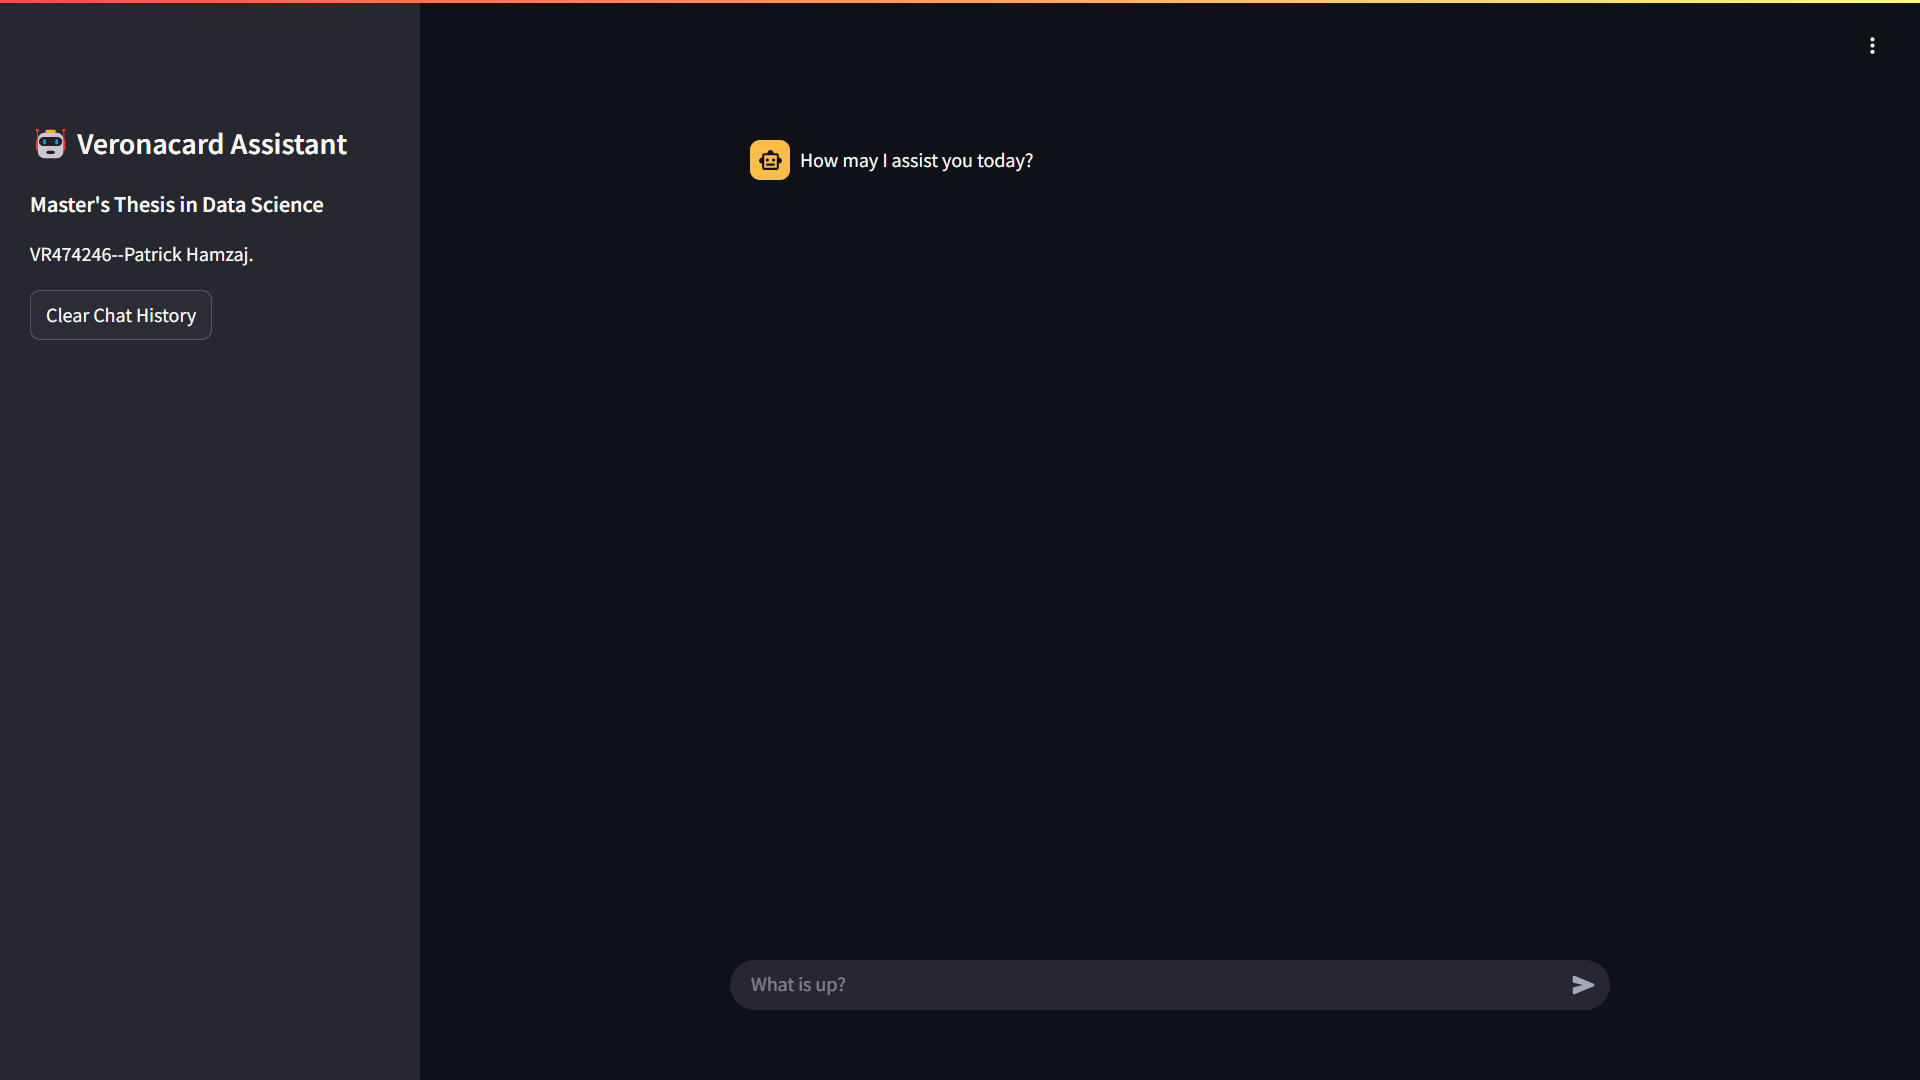
\includegraphics[width=1\textwidth]{images/streamlit-app.png}
    \caption{The front-end user interface.}
    \label{fig:streamlit-app}
\end{figure}

The front-end is presented as a clear and simple touch point that resembles commonly used chatbot products, as can be seen in Figure \ref{fig:streamlit-app}. The principal component is the user input, which can be typed into the message bar at the bottom of the page; this will be displayed in the main content, namely the chat, that hosts the multi-turn conversation between the user and the model. A concealable left sidebar has the purpose to present the project in few words, and permits to reinitialize the chat.

As soon as the send button is clicked (or the enter key is pressed), the app sends a POST to the Flask server's endpoint \verb|/predict|, loaded with a JSON formatted prompt. The object is then parsed and the user's prompt is then extracted in a raw format, appended to the backend chat history--this is not responsible for the visible front-end chat, but rather the context to be give to the model--and then given as a parameter to the \texttt{generate\_response(model, token, prompt)}.

\begin{center}
\begin{minipage}{0.7\textwidth}
\begin{lstlisting}[language=Python, frame=single, caption=Predict Flask API.]
# This decorator tells Flask to set it as a callable endpoint
@app.route('/predict', methods=['POST'])
# The function called as soon as the user sends a message
def predict():
    data = request.json
    prompt = data.get('prompt', '')
    messages.append({"role": "user", "content": prompt})
    response = generate_response(tokenizer, model, messages)
    messages.append({"role": "assistant", "content": response})
    return jsonify({"response": response})
\end{lstlisting}
\label{lst:predict-api}
\end{minipage}
\end{center}

This function is the engine of the LLM: it is a step-by-step procedure that orchestrates the internal functioning of the model, parsing the input with the tokenizer, moving the computation to the GPU, setting the temperature and the necessary number of tokens and finally triggering a response, which is now discussed in depth.

This function has four parameters:
\begin{enumerate}
    \item \textbf{tokenizer:} Is one of the two main characters in defininf the model, as seen in Section \ref{sec:tokenization} and implemented in Code \ref{lst:transformers-script}.
    \item \textbf{model:} The second main character, covering both architecture and checkpoints as seen in Section \ref{sec:transformer-architecture} and implemented in Code \ref{lst:transformers-script}.
    \item \textbf{messages:} The chat history between the model and the user. This is a list of dictionaries of the form \texttt{\{"role": System/User/Assistant, "content": The prompt\}}.
    \item \textbf{tool\_call:} Serves whenever a tool call is not conceived, as for example when performing few-shot and teaching the model when to use a tool and when not to use it.
\end{enumerate}

\begin{center}
\begin{lstlisting}[language=Python, frame=single, caption=\texttt{generate\_response()} Function.]
def generate_response(tokenizer, model, messages, tool_call=True):
    """
    Generates a response based on the provided prompt.

    Args:
        tokenizer: The tokenizer used to prepare the text.
        model: The LLaMa model.
        prompt: The initial prompt string.
        max_length: Maximum length of the generated text.

    Returns:
        A string containing the generated response.
    """

    # Define the set of tools the model can use
    tools = [retrieve_affluency]

    if not tool_call:
        tools = None

    # Takes the chat history, the set of tools and tells the model to return
    # a response as a dictionary
    inputs = tokenizer.apply_chat_template(
        messages,
        tools=tools,
        add_generation_prompt=True,
        return_dict=True,
        return_tensors="pt"
    )

    # Move inputs to the same device as the model (GPU)
    inputs = {key: tensor.to(model.device) for key, tensor in inputs.items()}

    # Generate the output given the input, how many tokens the model can use,
    # the temperature and select the top 50% tokens that are most probable
    output = model.generate(
        **inputs,
        max_new_tokens=512,
        temperature=0.5,
        top_p=0.5,
        do_sample=True
    )

    # Decode the output into human readable format
    response = tokenizer.decode(output[0][len(inputs["input_ids"][0]):], skip_special_tokens=True)

    # We handle the case when the model returns a tool call
    if response.startswith("{"):
        messages.append({"role": "assistant", "content": response})
        response = eval(response)

        # We extract the function called and the parameters set
        name = response['name']
        parameters = response['parameters']

        arguments = {k: v for k, v in parameters.items() if v is not None}

        tool_call = {"name": name, "arguments": arguments}
        messages.append({"role": "assistant", "tool_calls": [{"type": "function", "function": tool_call}]})

        # The retrieve_affluency function returns the output with the parsed arguments
        if name == "retrieve_affluency":
            content = retrieve_affluency(tool_call["arguments"]["location"], tool_call["arguments"]["date"])
        # elif name == "get_weather_forecast":
        #     content = get_weather_forecast(tool_call["arguments"]["date"])
        else:
            content = ""

        # The function's output is then appended to the chat history
        messages.append({"role": "tool", "name": name, "content": content})

        # From here on, the behaviour is the same as a standard conversation,
        # with the difference that the model now has to generate a response based on the 
        # function's output
        inputs = tokenizer.apply_chat_template(
            messages,
            tools=tools,
            add_generation_prompt=True,
            return_dict=True,
            return_tensors="pt"
        )

        inputs = {key: tensor.to(model.device) for key, tensor in inputs.items()}

        output = model.generate(
            **inputs,
            max_new_tokens=512,
            temperature=0.5,
            top_p=0.5,
            do_sample=True
        )

        response = tokenizer.decode(output[0][len(inputs["input_ids"][0]):], skip_special_tokens=True)

    return response
\end{lstlisting}
\end{center}

The set of tools that enable and agentic behaviour is defined, containing the \texttt{retrieve\_affluency()} function which points to the VeronaCard dataset and extracts affluency data based on day and time. The \textit{tokenizer} method \sloppy{\texttt{apply\_chat\_template()}} comes in aid when parsing human-form text: a chat template is a part of the tokenizer and it specifies how to convert conversations into a single tokenizable string in the expected model format. This is an example of LLaMa 3.1 8B Instruct model's required format:

\begin{Verbatim}[breaklines=true]
<|begin_of_text|><|start_header_id|>system<|end_header_id|>

Cutting Knowledge Date: December 2023
Today Date: 23 July 2024
    
You are a helpful assistant<|eot_id|><|start_header_id|>user<|end_header_id|>
    
What is the capital of France?<|eot_id|><|start_header_id|>assistant<|end_header_id|>
\end{Verbatim}

Different models have different chat formats, and it is important to set a chat template format that matches the template format a model was pretrained on. The above-mentioned method deals with selecting the right format for a given model under the hood, allowing to just input a dictionary with essential role-content keys.
Finally, this method takes as inputs the chat history, the tools enabling the agentic behaviour and a few more arguments that dictates the tokenizer's basic settings.
The \texttt{output} variable holds the model generated content, which sets also the \textit{temperature}, a value ranging from 0 to 1, determining the creativity or deterministic response, the maximum \textit{number of tokens} to genereate, a \textit{top\_p} parameter that indicates the most probable tokens to select. The \texttt{response} holds the decoded response of the model.

A normal interaction would return this final response, but the function also handles the case in which the generated response is not textual but, following the flow described in Section \ref{sec:agent-ai}, is a tool call. When this is the case, after parsing the content, it extracts the name of the tool and the parameteres captured by the model, to call the \texttt{retrieve\_affluency()} function in order to get the statistics regarding a specific point of interest in a specific day and time, suggesting to visit that attraction if feasible, otherwise recommending a less busy moment. It then proceeds to follow the precedent behaviour in applying the chat template, setting generation parameters and finally decoding and returning the response. The implementation of this function is given in Code \ref{lst:retrieve-affluency}.

\begin{center}
\begin{lstlisting}[language=Python, frame=single, caption=\texttt{retrieve\_affluency()} Function.]
def retrieve_affluency(location: str, date: str) -> str:
    """
    Get the current affluency of a specific location, based on past data.

    Args:
        location: The location to get the affluency data.
        date: The datetime to get the affluency data.

    Returns:
        The current affluency at the specified location.
    """

    if date:
        parsed_date = dateparser.parse(date)
        if parsed_date == None:
            parsed_date = timefhuman(date)

        hour = parsed_date.hour
        month = parsed_date.month
        weekday = parsed_date.weekday()
    else:
        today = datetime.now()
        month = today.month
        weekday = today.weekday()
        hour = today.hour

    prompt = is_location_crowded(location, month, weekday, hour)

    if "medium" in prompt or "high" in prompt:
        prompt += f'\nSuggest alternative time: {suggest_alternative_time(location, month, weekday)}.'

    return prompt
\end{lstlisting}
\label{lst:retrieve-affluency}
\end{center}

Tha main duty of this function is to parse the date and divides it into atomic parts, i.e. day, month, weekday and hour. It the proceeds to call another function, \texttt{is\_location\_crowded()}, that can be seen in Code \ref{lst:is-location-crowded}, which takes these newly forged data, along with the point of interest, and performs a series of operation on the VeronaCard dataset.

\begin{center}
\begin{lstlisting}[language=Python, frame=single, caption=\texttt{is\_location\_crowded()} Function.]
def is_location_crowded(location: str, month: int, weekday: int, hour: int) -> str:
    # Handled the case when the prompt does not require a specifice time,
    # rather only a date
    if hour == 0:
        df_location = df[(df['sito_nome'] == location) & (df['weekday'] == int(weekday))]
    # If the hour parsed is not present in the records, it implicitly means
    # that the site is closed
    elif hour not in df[(df["sito_nome"] == location) & (df["mese_visita"] == month)]["ora_visita_intervallo"].unique():
        return "The site is closed."
    # Otherwise, return all the records that correspond to the point of interest
    # in the specified datetime
    else:
        df_location = df[(df['sito_nome'] == location) & (df['weekday'] == int(weekday)) & (df['ora_visita_intervallo'] == int(hour))]

    # Perform some aggreagations in order to get monthly visits
    location_visits = df_location.groupby(['anno_visita', 'mese_visita', 'weekday', 'ora_visita_intervallo']).size().reset_index(name='visits_number')
    visits = location_visits.groupby(['mese_visita', 'weekday', 'ora_visita_intervallo'])['visits_number'].mean().reset_index(name='visits_mean')

    maps_ranking = visits[visits['mese_visita'] == month]
    # If we get one record, it means it must return a suggestion
    # incorporating also hour information we got in the arguments
    if len(maps_ranking) == 1:
        maps_ranking = maps_ranking['visits_mean'].iloc[0]
        # Calculates the percentile
        maps_percentile = (visits['visits_mean'] <= maps_ranking).mean() * 100
        prompt = f"Estimated affluency for {location}: "

        if maps_percentile <= 33:
            prompt += "low."
        elif maps_percentile <= 66:
            prompt += "medium."
        else:
            prompt += "high."

        return prompt
    # Otherwise, a precise suggestion is made, because user did not
    # give hour preference, but rather a generic recommendation
    else:
        try:
            maps_percentile = maps_ranking[maps_ranking["visits_mean"] < maps_ranking["visits_mean"].median()].sort_values(by="ora_visita_intervallo")["ora_visita_intervallo"].iloc[0]
            return f"Suggested time for {location}: {maps_percentile}."
        except IndexError:
            return "The site is closed."
\end{lstlisting}
\label{lst:is-location-crowded}
\end{center}

\texttt{is\_location\_crowded()} takes the atomic data chunked by the \texttt{retrieve\_affluency()} and performs a series of operation in order to gather affluency data. In particular, it handles three cases: when user asks for recommendation for today, tomorrow or generally a time window, the parser sets \textit{hour} to 0, and that is the sign to give a suggestion solely based on the \textit{date} parameter (e.g., \textit{What time should I visit Arena today?}), returning a suggested time for visiting; if hour information is given, then it proceeds to check if it present in the dataset for that specific point of interest--if not the site should be labeled as closed. Finally, if all information is given, namely the attraction, month, weekday and hour (e.g. \textit{I would like to visit Castelvecchio tomorrow at 3pm.}), the function returns an estimation of the turnout calculating the mean of the number of visits in that weekday for that specific month, across all months, based on the percentile that specific time belongs to, allowing for three values to be appended to the prompt (\textit{low}, \textit{medium}, \textit{high}).

Subsequently, as can be seen in Code \ref{lst:retrieve-affluency}, if the estimated afflunecy is not low, it provides an alternative time, which may provide less crowded visiting moments, implemented through Code \ref{lst:suggest-alternative-time}.

\begin{center}
\begin{lstlisting}[language=Python, frame=single, caption=\texttt{suggest\_alternative\_time()} Function.]
def suggest_alternative_time(location: str, month: int, weekday: int) -> str:
    # It performs similar operations of is_location_crowded function,
    # but it returns the median value of the vists across the
    # weekdays of the month, across all months
    df_location = df[(df['sito_nome'] == location) & (df['weekday'] == int(weekday)) & (df['mese_visita'] == int(month))]
    location_day = df_location.groupby(['anno_visita', 'mese_visita', 'weekday', 'ora_visita_intervallo']).size().reset_index(name='visit_count')
    hours_affluency = location_day.groupby('ora_visita_intervallo')['visit_count'].agg(lambda x: x.mean()).reset_index(name='mean_visits')

    # Less crowded time to visit the attraction
    alternative = hours_affluency.median()

    return int(alternative['ora_visita_intervallo'])
\end{lstlisting}
\label{lst:suggest-alternative-time}
\end{center}

This utility performs similar operations to the \texttt{is\_location\_crowded()} function in gathering affluency data by weekday and month across all months, but this time it returns the median value for that day in order to provide a lower crowded moment to suggest to the user.

After having outlined both the operational settings as importing the LLM's architecture and checkpoints, importing the tokenizer with appropriate parameters, instatiate the model, and having described the set of tools enabling the dyanmic behaviour of the model, the instance of the context enabling the domain-specific expertise seen in Sections \ref{sec:prompt-engineering} and \ref{sec:agent-ai} shall be discussed.

In order to augment model's knowledge, the \texttt{message} variable have been enhanced with the \texttt{SYSTEM} prompt discussed in Section \ref{sec:prompt-anatomy}. The system prompt has been crafted outlining the model's role, thus directing the model's response tone and focusing on relevant outcomes, as seen in Section \ref{sec:role-prompting}:

\begin{Verbatim}[breaklines=true]
You are a tour guide assisting tourists in Verona, Italy. Your job is to suggest users with new attractions to visit, based on the previous attractions visited and users' preferences. Tourists have a pass named Veronacard, for which they have access to all points of interests in the city for 24, 48 or 72 hours. Your tone is both professional and friendly at the same time.
\end{Verbatim}

Some indications about the role that the model must adopt were given, namely that he is a tour guide that assists tourist, also giving instruction about the tone to take, which must be \textit{both professional and friendly at the same time}.
Afterwards, to obtain a factual knowledge that increased the model's actual knowledge derived from the training phase, a basic RAG approach--seen in Section \ref{sec:rag}-- was adopted, injecting the relevant information directly under the previus data:

\begin{Verbatim}[breaklines=true]
Today's date is Wednesday, 22 January 2025.
The weather throughout the day is as follows:
At 07:00 the temperature is 5°C with fog. The precipitation probability is 0%.
At 08:00 the temperature is 5°C with fog. The precipitation probability is 0%.
At 09:00 the temperature is 5°C with fog. The precipitation probability is 0%.
At 10:00 the temperature is 6°C with fog. The precipitation probability is 0%.
At 11:00 the temperature is 6°C with fog. The precipitation probability is 13%.
At 12:00 the temperature is 7°C with slight rain. The precipitation probability is 43%.
At 13:00 the temperature is 7°C with slight rain. The precipitation probability is 63%.
At 14:00 the temperature is 8°C with overcast. The precipitation probability is 68%.
At 15:00 the temperature is 8°C with overcast. The precipitation probability is 78%.
At 16:00 the temperature is 8°C with slight rain. The precipitation probability is 93%.
At 17:00 the temperature is 7°C with moderate drizzle. The precipitation probability is 93%.
At 18:00 the temperature is 7°C with slight rain. The precipitation probability is 75%.
At 19:00 the temperature is 7°C with slight rain. The precipitation probability is 35%.
At 20:00 the temperature is 6°C with slight rain. The precipitation probability is 23%.
You must suggest users on attractions to visit included in the Veronacard, which are the following: 
- AMO
- Arena
- Casa Giulietta
- Castelvecchio
- Centro Fotografia
- Duomo
- Giardino Giusti
- Museo Africano
- Museo Conte
- Museo Lapidario
- Museo Miniscalchi
- Museo Radio
- Museo Storia
- Palazzo della Ragione
- San Fermo
- San Zeno
- Santa Anastasia
- Sighseeing
- Teatro Romano
- Tomba Giulietta
- Torre Lamberti
- Verona Tour
\end{Verbatim}

In the training phase, models have a cut-off knowledge to a specific date, which must be overwritten by explicitly declaring the actual date--if not declared, the model may respond with outdated or corrupted information--for LLaMa 3.1 8B Instruct the knowledge cut-off date is Decembre 2023. The weather information is retrieved and injected dinamically based on the current date, and is mapped hourly, indicating the temperature, a weather condition (e.g., \textit{slight rain}) and a precipitation probability. The same applies to the points of interest to suggest: the attraction are taken for unique \texttt{sito\_nome} of the VeronaCard dataset, which is statically retrieved (the dataset does not change).
Finally, indications about the tools available to the model are given, allowing for an Agentic behaviour described in Section \ref{sec:agent-ai}:

\begin{Verbatim}[breaklines=true]
You can call the function retrieve_affluency whenever the user wants information on the affluency of a specific location; in all other cases you should respond naturally. Include weather data whenever the user asks for suggestions, so that for example you can recommend indoor places when it is rainy and outdoor places when it is sunny.
\end{Verbatim}

As can be noted, instructions about when to call the tool available and how to use weather data were given, in order to better direct the model's response. To further enhance the model's comprehension of the type of interactions desired, its native capability of \textit{few-shot} learning, as seen in Section \ref{sec:prompt-engineering} has been engaged. In particular, an example of a generated natural response was given first, then a second example involving the tool call for affluency data, as given below:

\begin{Verbatim}[breaklines=true]
\underline{USER}:       Hey, what attraction should I visit?

\underline{ASSISTANT}:  Buongiorno! Welcome to Verona. I'd be happy to help you plan your day. Considering you've already visited some of the most popular attractions like the Arena, Casa Giulietta, and Castelvecchio, I'd like to suggest some other places that might interest you.

However, I need to know a bit more about your preferences. Are you interested in history, art, architecture, or something else? And would you like to visit indoor or outdoor attractions?

Also, I should let you know that the weather today is quite rainy, with a high chance of precipitation. So, if you'd like to stay dry, I can recommend some indoor attractions.

Let me know your preferences, and I'll do my best to suggest some great places to visit!
\end{Verbatim}

The user's prompt was hard-coded, while the assistant's response was generated by the model, setting the parameter \texttt{tool\_call=False} in the generation function \texttt{generate\_response()}, so that to teach the model to respond naturally when no crowd-based suggestion is requested. Thereafter, an example of the tool call to \texttt{retrieve\_affluency()} was given:

\begin{Verbatim}[breaklines=true]
\underline{USER}:       I don't want too many crowds, what time would you suggest for visiting Giardino Giusti today?
\end{Verbatim}

The model's output then follows the steps described in Section \ref{sec:agent-ai}:

\begin{center}
\begin{minipage}{0.7\textwidth}
\begin{lstlisting}[language=Python, frame=single, caption=Tool call]
# Tool call
{
    'role': 'assistant',
    'tool_calls': [
        {
            'type': 'function',
            'function': {
                'name': 'retrieve_affluency',
                'arguments': {
                    'location': 'Giardino Giusti',
                    'date': '2025-01-22'
                }
            }
        }
    ]
},

# Function's output
{
    'role': 'tool',
    'name': 'retrieve_affluency',
    'content': 'Suggested time for Giardino Giusti: 8.'
}
\end{lstlisting}
\end{minipage}
\end{center}

Which finally gives a response to the users's prompt:

\begin{Verbatim}[breaklines=true]
\underline{ASSISTANT}:  Considering the weather forecast for today, which is mostly overcast with a slight chance of rain in the evening, I suggest visiting Giardino Giusti at 8:00 AM. This should give you a chance to avoid the crowds and enjoy the peaceful atmosphere of the garden before the day gets busy.
\end{Verbatim}

The resulting behaviour coherently maintained throughout the conversation, which overall makes prompt engineering a useful feature to leverage without incurring in expensive setups, for delivering natural and domain-specific interactions with a low-rank model such as LLaMa 3.1 8B Instruct. The following chapter provides an extensive set of meaningful conversations held, in order to give an evaluation of the effectiveness of the strategies adopted in the project.